\setcounter{figure}{0}
\setcounter{table}{0}
\setcounter{footnote}{0}

\articletitle{Child Trafficking in India: An Overview}\label{2016-art5}

\vspace{-.3cm}

\articleauthor{Avanish Bhai Patel\footnote{PhD Scholar, IIT Roorkee, Uttarakhand}}
\lhead[\textit{\textsf{Avanish Bhai Patel}}]{}
\rhead[]{\textit{\textsf{Child Trafficking in India:....}}}



\begin{multicols}{2}

\heading{Introduction}

\noi
Trafficking of human beings, particularly children, has emerged as a matter of grave concern around the world, including in India, in recent years. It is the most serious form of organized crime in the world, and it cuts across cultures, geographies, and time periods (INTERPOL, 2005). “Human Trafficking is the recruitment, transportation, transfer, harbouring or receipt of people through force, fraud or deception, with the aim of exploiting them for profit” (United Nations, 2002). Human trafficking is also an unauthorised trade in human beings for the purpose of reproductive enslavement, commercial sexual exploitation, forced labour, and other forms of exploitation, among other things. (United Nations, 2008). The practice of human trafficking is referred to be a modern-day variant of slavery since it takes place in the contemporary world (INTERPOL, 2005; Stop the Traffick, 2006). Although the precise number of persons enticed or coerced over international boundaries each year is unclear, even conservative estimates show that at least 2.5 million children, women, and men are trafficked and forced to work in dismal and risky conditions against their will (Johannes Koettl, 2009). Many more are trafficked and forced to work within their own countries, often under dubious and dangerous conditions and held captive by physical, psychological or financial threats (Johannes Koettl, 2009). It is the truth that human trafficking is an abhorrent assault to the dignity and rights of those who are trafficked. It has been estimated that out of the total number of persons affected by human trafficking in which 80\% women and 50\% children are affected by human trafficking in India (P.P.I., 2010). Moreover, annually, 20 billion rupees are turned over through human trafficking (P.P.I., 2010). For thousands of men, women, and children, India is a source of resources, a transit point, and a destination (Sen, 2003; Srivastava, 2007; P.P.I., 2010). India's frontier states have a common border with neighboring nations such as Nepal, Bangladesh, China, Pakistan, and others (Shrivastava, 2007 and Sharma, 2007). The children from these nations are readily accepted for commercial sex in these countries (Sharma, 2007; P.P.I., 2010).

\noi
Trafficking of children is the most alarming issue around the globe today. Many girl
children in India are involved in commercial sex as a result of religious prostitution,
sex tourism, and pornographic material (Sen, 2003; Manzo, 2005; Sharma, 2007). In a
nutshell, religious prostitution is referred to as devadasi pratha in India, and it is socially
acceptable in some sections of the country (Sen, 2003; Shrivastava, 2007). Religious
prostitution can be found in Andhra Pradesh, Karnataka, Tamil Nadu, Kerala, and
Maharashtra, among other places of worship (Sen, 2003, Nair, 2007, Ray, 2007). Sex
tourism may be defined as visits planned inside the tourism industry or outside the
business but exploiting its structures and networks, with the main objective of
promoting a commercial sexual connection between the tourist and the people of a
specific place (World Tourism Organisation, 1995). Pornography is also the most
dangerous kind of human trafficking, coming in second only to sex tourism. Sex
traffickers (sex tourists) are in the forefront of the production of pornographic content,
which includes images, films, and videos of nude children, as well as sex with the
children themselves. Traffickers are frequently found to be involved in the production,
collection, and distribution of pornographic material (Sen, 2003; Nair, 2007; Roy,
2013).

\noi
Esquibel (2005) has pointed out in her research that trafficked individuals are either
underpaid or get inadequate compensation. As a commodity, they may be resold again
and over again for a profit, and they can be utilised to accumulate wealth. Traffickers
deceive migrants into believing that they would be able to make many times more
money overseas than they are able to earn in their native country. Furthermore, he
asserts that the rise in global poverty has resulted in the establishment of worldwide
human trafficking. Similarly, Manzo (2005) has indicated in his research that poverty
is the primary cause of human trafficking. Trafficking thrives in areas where poverty
reflects a more widespread systemic issue. Whereas children are more likely to emigrate
to find work away from their parents. He has also emphasised that there is a close
connection between poverty and human trafficking. Furthermore, Sharma (2007) has
done her research on human trafficking in the state of Maharashtra. In her research, she
has found that human trafficking is a blatant violation of basic rights, and she concluded
that it is. It also infringes the right to health and health care, the right to liberty and security of person, as well as the right to be free from torture, assault, cruelty, or
humiliating treatment or punishment. The trade and exploitation of human beings is the
most heinous violation of human rights committed by traffickers and organised crime
groups. To add to this, in order to explain human trafficking, Lutya (2009) proposed an
epi-criminological theory based on two distinct fields, public health and criminal justice
to examine human trafficking. He has tackled South African human trafficking of
young women and girls for the purpose of compelled prostitution via a scholarly
synthesis of epistemological and criminal justice solutions. From the preceding lines it
is apparent that human trafficking is prevailing among the children in India and
therefore, there is a dire need of scientific enquiry to analyse this issue from multiple
perspectives and explore the factors which are responsible for trafficking among the
women and children.

\subsection*{Multiple Factor School of Criminology and Child Trafficking:}

\noi
Criminologists
have made use of multiple factor school to define the factors of crime. The followers
of this school believe that crime is the outcome of a combination of many variables
which cannot be stated in terms of general premise. According to this school there are
so many variables of committing crime and it illustrates this fact in the context of
causality of crime that no scientific theory of criminal behavior is possible
(Chaturvedi, 2007). Ferrie asserts that crime is the outcome of a variety of
circumstances in his discussion of crime (Sutherland and Cressey, 2011; Chaturvedi,
2007). These circumstances are closely related to one another, and by doing a thorough
investigation, these factors can be discovered in the society. There are three types of
factors: social, natural, and anthropological. Furthermore, according to American
criminologist William Healy, it is not one or two circumstances that cause a man to
become a delinquent, but rather a mixture of several elements that together drive him
to engage in criminal behavior (Sutherland and Cressey, 2011). Migration, culture
conflicts, familial background, political ideology, religion and crime, economic
situations, and the ecology of crime are some of the aspects to consider (Paranjape,
2011). Furthermore, he contends that not all of the circumstances linked with a given
crime are of equal importance as a contributing factor to the commission of that crime.
It is impossible to understand criminal behavior without first gathering all of the
relevant information.
\end{multicols}
\begin{figure}
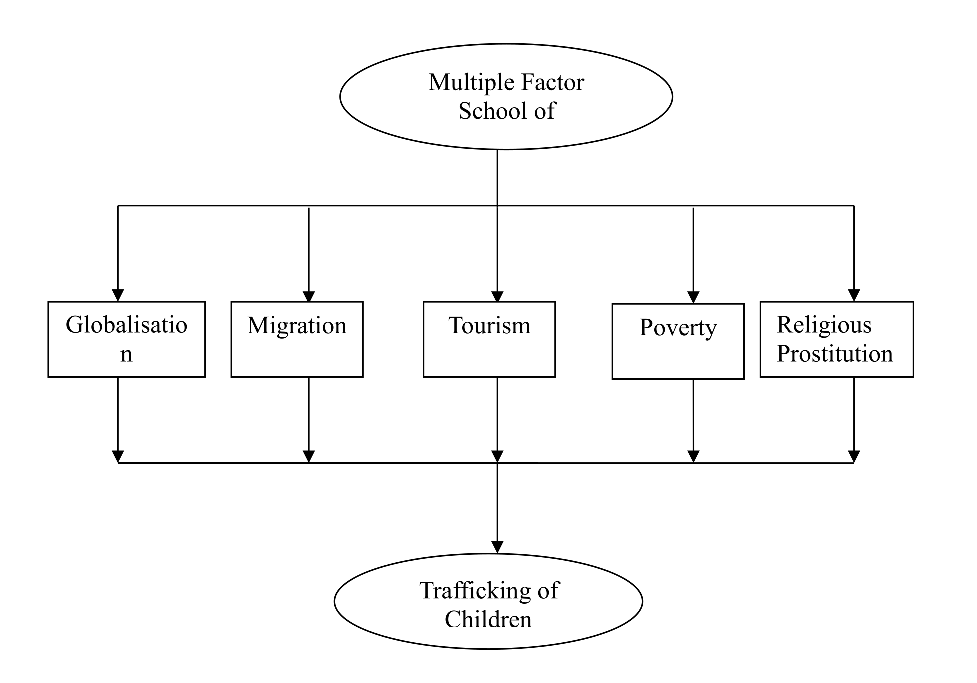
\includegraphics[scale=1.1]{images/fig001.eps}
\end{figure}

\vspace{-.3cm}

\begin{multicols}{2}

\noi
So for now, we've talked about the multiple factor school of criminology and how
numerous factors influence the decision to commit a crime. With the assistance of the
multiple factor school, we will now investigate the factors that contribute to human
trafficking. It is no longer possible to assess any social phenomenon on the basis of just
one or two components in the modern day. The occurrence of each social phenomenon
is influenced by a variety of circumstances. A similar result is obtained when we
examine child trafficking using the multiple factor school of crime, which reveals that
a variety of causes are at the root of the problem. Poverty, tourism, migration, religious
prostitution, globalization, corruption, illiteracy, and lax law enforcement are just a few
of the variables that influence people's lives.

\noi
\textbf{Objective :} the objective of paper is to understand the nature and extent of child
trafficking in India. The paper also examines the causes of child trafficking under the
multiple factor school of criminology.

\noi
\textbf{Data Sources :} This study is based on secondary data. Secondary data have been
collected from Crime in Report, 2015 which is published by National Crime Record
Bureau. A starting point for the analysis of available data is National Crime Record
Bureau that collects data on trafficking through State Crime record Bureaus and Union Territories. These data provide an indication of the level or reporting of trafficking
within India.

\vspace{-.4cm}

\subsection*{Result and Discussion:}

\vspace{-.2cm}

\noi
\textbf{Registered Cases of Child Trafficking in Indian Penal Code and Special Laws:} A
total of 3490 incidents of child trafficking under various provisions of laws relating to
human trafficking have been reported in the country during 2015. The cases related to
human trafficking grew from 0.4 percent in 2014 to 0.5 percent throughout the course
of the year 2015. During the years 2011–2015, there has been an increase in the number
of reported cases of human trafficking. During 2011, a total of 3,517 cases were
reported, with the number increasing to 3,554 cases in 2012, 3,940 cases in 2013, 5,466
cases in 2014, and 6,877 (in which 3490 cases of child trafficking) cases in 2015.

\noi
\textbf{Immoral Traffic (Prevention) Act, 1956 :} A total of 58 cases under the Immoral
Traffic (P) Act were registered in the country. Majority of these cases were reported in
Maharashtra (18 cases) and Karnataka (10 cases) and West Bengal (9 cases) during
2015. These States together accounted for 63.8\%(37 out of 58 cases) of total child
trafficking under this Act during 2015.

\noi
Human Trafficking under Section 370 and 370 A IPC: During the year 2015, a total of
221 incidents of child trafficking under the provisions of sections 370 and 370A of the
Indian Penal Code were reported across the nation. There have been 57 reports of
similar occurrences in Delhi, followed by Bihar (27 reports), Madhya Pradesh (22
reports), Odisha (20 reports), West Bengal (15 reports), Chhattisgarh (12 reports), and
Telangana (one complaint) (11 cases). During the year 2015, these states together
accounted for 72.4 percent of all violent crimes.

\noi
\textbf{Other Various Cases of Child Trafficking under IPC Sections: Importation of
Girls (Section 366-(B) I.P.C.):} A total of 2 cases of importation of girls from foreign
country were registered during 2015. Uttarakhand and West Bengal has reported 1 case
each during 2015. \textbf{Procuration of Minor Girls (Section 366-(A) I.P.C.):} A total of
3087 cases have been reported in 2015. \textbf{Selling of Girls for Prostitution (Section 372
I.P.C.):} There have been 111 cases reported in the country during 2015. \textbf{Buying of
Girls for Prostitution (Section 373 I.P.C.):} There have been 11 cases reported in
country during 2015.

\noi
\textbf{Nature and Problem of Human Trafficking:} Various forms of child trafficking
include child labour, early marriage, sexual assault, begging and organ trade etc. The
girl children are trafficked from rural regions and utilised as street sellers or domestic
employees by persons in metropolitan areas (Manzo, 2005). There are a variety of
employment opportunities for exploited children in India due to human trafficking
(UNHR, 2014; Sahariahi, 2015). They are exploited in industries and farms, in brothels
and houses, and are compelled to work as smugglers and beggars to survive (Sen, 2003;
Ray, 2007, Roy, 2013). Commercial matchmakers need the girls to keep their agencies
going and children are forced to labour to pay off their parents' debts, and they often
spend years of their lives in slavery (Sen, 2003; Roy, 2013; Sahariahi, 2015). In addition
to sex trade activities such as sex tourism and pornography (Sen, 2003; UNHR, 2014),
a large number of children are trafficked for other forms of non-sex-based exploitation,
which include servitude of various kinds, such as domestic or factory work or farming,
begging, organ trade, and false marriages (Ray, 2007; Roy, 2013). The number of
minors being trafficked is increasing, and over 60\% of those who are victims of
trafficking are under the age of 18. (N.C.R.B., 2005). In India, it is believed that there
are more than 9,000,000 sex workers and approximately, 30\% are believed to be
children. According to recent statistics, the number of minors engaging in prostitution
is growing at a rate of 8\% to 10\% every year, on average (Shrivastava, 2007).

\noi
A large number of children are victims of forced labour, begging and sexual
exploitation. Innocent children, boys and girls are exposed to vulnerable situations,
violence and sexual abuse. This is a violation of human rights and children are deprived
(Ray, 2007; UNHR, 2014). It disturbs the mental and physical capacity of the child
which is primary for the development of every child (Sen, 2003, Shrivastava, 2007;
UNHR, 2014). Children lose their childhood due to the malpractices of child trafficking
(Sahariahi, 2015). Children are robbed of their basic rights, irrespective of economic
status, caste, and gender (Ray, 2007; UNHR, 2014). Traffickers know children have
less developed mental capacity to understand right and wrong and are less able to
handle their trauma as compared to adults (UNHR, 2014).

\noi
\textbf{Conclusion:} A framework for analysing the many circumstances and types of slavery
that contribute to the trafficking of children in India is provided by the study. Several
reasons have been identified as contributing to child trafficking, but poverty, tourism,
migration have received the most attention in this research, which concludes that there 
are several. These are the kinds of conditions that make individuals more vulnerable to
being victims of human trafficking. According to the study, the number of incidents of
child trafficking in the nation is rapidly growing. Significantly, child trafficking is done
for organ trafficking, sexual abuse and child labor. There are no very effective laws in
the direction of prevention of child trafficking in India. Although some laws have been
made in this area but they are insufficient as they are not strict. Illegal trade in human
beings or persons is prohibited under Article 23 of the Constitution of India. Immoral
Trafficking Prevention Act and POCSO Act are effective in child trafficking law in
India. Human trafficking was made completely illegal in India in the year 1956. Various
provisions are made by the Ministry of Women and Child Development from time to
time to prevent child trafficking.

\noi
Last but not least, I would like to say that it is up to all of us intelligent citizens to fulfil
our duty and responsibility in order to bring this serious and sensitive problem under
control, so that the young children of today can breathe freely in this democratic country
and live their childhoods with dignity, allowing them to experience the joys of
childhood.


\end{multicols}
\label{end2016-art5}
